% This must be in the first 5 lines to tell arXiv to use pdfLaTeX, which is strongly recommended.
\pdfoutput=1
% In particular, the hyperref package requires pdfLaTeX in order to break URLs across lines.

\documentclass[11pt]{article}

% Remove the "review" option to generate the final version.
\usepackage[]{acl}

% Standard package includes
\usepackage{times}
\usepackage{latexsym}

% For proper rendering and hyphenation of words containing Latin characters (including in bib files)
\usepackage[T1]{fontenc}
% For Vietnamese characters
% \usepackage[T5]{fontenc}
% See https://www.latex-project.org/help/documentation/encguide.pdf for other character sets

% This assumes your files are encoded as UTF8
\usepackage[utf8]{inputenc}

% This is not strictly necessary, and may be commented out,
% but it will improve the layout of the manuscript,
% and will typically save some space.
\usepackage{microtype}


% added by lemon
\usepackage{algorithmicx}  
\usepackage{algpseudocode}  
\usepackage{amsmath}  
\usepackage{color,xcolor}
\usepackage{algorithm} %format of the algorithm 
\usepackage{pifont}
\usepackage{bm}
\usepackage{amsfonts}
\usepackage{graphicx}
\usepackage[normalem]{ulem}
\usepackage{multirow}
\usepackage{url}
\usepackage{tikz}
% \usepackage{subfigure}
\usepackage{xcolor}
\usepackage{tcolorbox}
\usepackage{color,xcolor}
\usepackage{amssymb}
\usepackage{amsopn}
% \usepackage{subcaption}
\usepackage{graphicx}
\usepackage{multirow}
\usepackage[english]{babel}
\usepackage{bm}
%\DeclareMathOperator*{\argmin}{argmin}
\usepackage{array}
\usepackage{setspace}
\usepackage{todonotes}
\usepackage{xspace}
\usepackage{amsfonts}
\usepackage{array,multirow}
\usepackage{pgfplots}
\usepackage{tikz}
\usepackage{verbatim}
\usepackage{subfig}
\usepackage{arydshln}
\usepackage{booktabs}


% If the title and author information does not fit in the area allocated, uncomment the following
%
%\setlength\titlebox{<dim>}
%
% and set <dim> to something 5cm or larger.

\title{DualNER: A Dual-Teaching framework for Zero-shot Cross-lingual Named Entity Recognition}

% Author information can be set in various styles:
% For several authors from the same institution:
% \author{Author 1 \and ... \and Author n \\
%         Address line \\ ... \\ Address line}
% if the names do not fit well on one line use
%         Author 1 \\ {\bf Author 2} \\ ... \\ {\bf Author n} \\
% For authors from different institutions:
% \author{Author 1 \\ Address line \\  ... \\ Address line
%         \And  ... \And
%         Author n \\ Address line \\ ... \\ Address line}
% To start a seperate ``row'' of authors use \AND, as in
% \author{Author 1 \\ Address line \\  ... \\ Address line
%         \AND
%         Author 2 \\ Address line \\ ... \\ Address line \And
%         Author 3 \\ Address line \\ ... \\ Address line}
\author{Jiali Zeng$^{1}\thanks{\ \ Corresponding author.}$, \ Yufan Jiang$^{1}$, \  Yongjing Yin$^{2}$, \ Xu Wang$^{1}$, \ Binghuai Lin$^{1}$, \ Yunbo Cao$^{1}$ \\
$^{1}$Tencent Cloud Xiaowei, Beijing, China \\
$^{2}$Zhejiang University, Westlake University, Zhejiang, China\\
{\tt \{lemonzeng,garyyfjiang,frostwu,ethanlli\}@tencent.com} \\
{\tt yinyongjing@westlake.edu.cn} \\ 
}
% \author{First Author \\
%   Affiliation / Address line 1 \\
%   Affiliation / Address line 2 \\
%   Affiliation / Address line 3 \\
%   \texttt{email@domain} \\\And
%   Second Author \\
%   Affiliation / Address line 1 \\
%   Affiliation / Address line 2 \\
%   Affiliation / Address line 3 \\
%   \texttt{email@domain} \\}

\begin{document}
% \pgfplotsset{compat=1.18}

\maketitle

\begin{abstract}

% Prior works in cross-lingual named entity recognition (NER) with no/little labeled data fall into two primary categories: model transfer based and data transfer based methods.
% The key points of the success of data transfer based methods is severely affected by the unsatisfactory quality of translation and the unpresision
% The performance of zero-shot cross-lingual Named Entity  Recognition (NER) is severely affected by the unsatisfactory quality of translation or label projection.
% This paper addresses zero-shot transfer for cross-lingual NER with a large amount of unlabeled target-language training data.
% We present a simple but effective data augmentation framework with a large amount of unlabeled target-language training data.
% by making complementary advantages of systems based on different paradigms.
% Recently,
% Predominantly, 
% two paradigms are used for NER tasks: Sequence Labeling and Span Prediction.
% Sequence labeling based models are better at dealing with those entities that are long and with low label consistency, while span prediction based models do better in sentences with more Out-of-Vocabulary (OOV) words and entities with medium length.
% Motivated by this, we 
% present a simple but effective data augmentation framework to combines the two learning paradigms.
% with a large amount of unlabeled target-language training data.
% we first 
% propose to combine the two learning paradigms into a joint framework and optimize it by two-stage training.
% Zero-shot cross-lingual named entity recognition (NER) is a challenging problem.
% Most of prior studies address the problem by constructing high quality pseudo target language corpus via satisfied machine translation model and complex label projection pipeline.
% Prior works in cross-lingual named entity recognition (NER) with no/little labeled data fall into two primary categories: data transfer and model transfer.
% Particularly,
% the performance of data transfer is severely affected by the unsatisfactory quality of translation and the inaccurate label projection.
% In this paper, we offer a simple but effective framework, coined DualNER, to utilize annotated source language corpus and unlabeled target language text without any translation model and label projection.
We present DualNER, a simple and effective framework to make full use of both annotated source language corpus and unlabeled target language text for zero-shot cross-lingual named entity recognition (NER).
% generate pseudo labels of the target language text without translation and label projection.
% to generate pseudo target-language corpus instead of translation with complex label projection.
% In particular, we combine two learning paradigms of NER into a joint framework to make complementary advantages of different paradigms. 
In particular, we combine two complementary learning paradigms of NER, i.e., sequence labeling and span prediction, into a unified multi-task framework.
% to make complementary advantages of them.
% As a start point,
% we simultaneously learn NER task in two task formulations
% via multitask learning 
% with annotated source language corpus.
% Then, given unlabeled target language text, one task formulation will produce pseudo-labels which are used as learning signals for the other task formulation.
% To achieve zero-shot cross-language NER, 
% We first optimize the framework
% by multi-task learning on annotated source corpus.
After obtaining a sufficient NER model trained on the source data, we further train it on the target data in a {\it dual-teaching} manner, in which the pseudo-labels for one task are constructed from the prediction of the other task.
% and vice versa
% jointly exploiting the two
% mainstream NER
% formulations on annotated source corpus, 
% Then, we propose a {\it dual-teaching} loss, which learns one task with the pseudo-labels for text in the target language constructed from the prediction of the other task, and vice versa.
% and then propose a {\it dual-teaching} loss for training on unlabeled target data.
% However, 
% use the trained model to generate pseudo-labels for each learning paradigm in a dual manner on unlabeled target data.
% Furthermore, we propose an entity-aware regularization to enhance the intrinsic cross-lingual alignment between the same entities in different languages.
Moreover, based on the span prediction, an entity-aware regularization is proposed to enhance the intrinsic cross-lingual alignment between the same entities in different languages.
% via an entity-aware regularization.
Experiments and analysis demonstrate the effectiveness of our DualNER.
Code is available at https://github.com/lemon0830/dualNER.
% It achieves a new state-of-the-art on the cross-lingual NER task.
% .proposed framework achieves new state of the art on cross-lingual NER without any label projection engineering.

\end{abstract}

\section{Introduction}

% Named entity recognition (NER) focuses on recognizing entities from raw text into predefined types \cite{}, which is an essential component for downstream natural language processing (NLP) tasks, such as information retrieval and question answering.
% However, most of the existing methods are highly dependent on the annotated training data and do not perform well in low-resource languages.
% Moreover, it is usually expensive and time-consuming to annotate such low-resource languages.
Aiming at classifying entities in un-structured text into pre-defined categories, named entity recognition (NER) is an indispensable component for various downstream neural language processing applications such as information retrieval \cite{banerjee-etal-2019-information} and question answering \cite{fabbri-etal-2020-template}.
Current supervised methods have achieved great success
% in a supervised setting 
with sufficient manually labeled data,
but 
% However, 
the fact remains that most of the annotated data are constructed for high-resource languages like English and Chinese, posing a big challenge to low-resource scenarios \cite{mayhew-etal-2017-cheap,bari-etal-2021-uxla}.

% and can be divided into two main categories:
% 1) model transfer with aligned cross-lingual word representations or pretrained multilingual language models \cite{conneau-etal-2020-unsupervised,bari-etal-2021-uxla}, which can not exploit the task-related information in the target language;
% 2) data transfer with machine translation and label projection \cite{mayhew-etal-2017-cheap,jain-etal-2019-entity,liu-etal-2021-mulda}.
% For the latter, the performance is severely affected by the unsatisfactory quality of translation and inaccurate label projection.
% Recently, knowledge distillation \cite{} is introduced to unify the data transfer and model transfer, which leverages large unlabeled data in the target language to further boost the cross-lingual NER performance \cite{wu-etal-2020-unitrans,fu-etal-2022-dual}.

To address this issue,
% the lack of training data in low-resource languages, 
zero-shot cross-lingual NER is proposed to transfer knowledge of NER from high-resource languages to low-resource languages.
% The knowledge can be transferred in either of the following two ways: 
The knowledge can be acquired in either of the following two ways: 
1) from aligned cross-lingual word representations or multilingual pre-trained encoder fine-tuned on high-resource languages
% , often English 
\cite{conneau-etal-2020-unsupervised,bari-etal-2021-uxla}.
2) from translated target language data with label projection \cite{mayhew-etal-2017-cheap,jain-etal-2019-entity,liu-etal-2021-mulda}.
These two kinds of methods can be unified into a knowledge distillation (KD) framework, to further improve the cross-lingual NER performance \cite{wu-etal-2020-unitrans,fu-etal-2022-dual}.
Though widely used, the transfer process still suffers from poor translation quality, label projection error and  over-fitting of large-scale multilingual language models. 
% In this paper, we present a simple and effective framework, named DualNER, 
% Unlike previous studies, we do not solve the above problems directly.
% Instead, we believe accurate 

In this paper, we present a simple and effective framework, named DualNER, alleviating the above problems from a different angle.
We combine two popular complementary learning paradigms of NER, sequence labeling and span prediction, into a single framework.
Specifically, we first train a teacher NER model by jointly exploiting sequence labeling and span prediction with the annotated source language corpus. 
Unlike the previous KD-based methods
% we do not produce pseudo-labels directly from correspond paradigms.
that produce pseudo labels for the corresponding paradigms,
% Instead, we present a dual-teaching strategy to make two paradigms complement each other, 
we propose a dual-teaching strategy to make the two paradigms complement each other.
More concretely, the model prediction
% inference probabilities 
for sequence labeling is used to construct the pseudo-labels for span prediction and vice versa.
% Previous studies can be divided into two categories:
% Some methods leverage the cross-lingual representations \cite{}, where the NER model is trained on the labeled corpus of the source language and then directly evaluated on target languages.
% Due to the success of multilingual pretrained language models \cite{}, these model-based transfer methods have shown a significant improvement on cross-lingual NER.
% Another line of research is the data-based transfer \cite{}, which adopts word-to-word translation to project the cross-lingual NER labels.
% For example, \cite{} employ a multilingual translation model with placeholders for label projection.
% Nevertheless, these methods are still limited by weak entity projection and do not leverage the unlabeled corpora in target languages.
% In this paper, we follow this research line and propose a simple yet effective framework, named DualNER, utilizing unlabeled target language text but without any translation model and label projection.
% Particularly, our DualNER unifies sequence labeling and span prediction via multi-task learning.
% is a multitask framework, which learns NER prediction via two task formulations.
% One task formulation constructs NER as a sequence labeling task.
% and assign label for each token.
% While the other formulates NER as a span prediction task.
% and extract entity span by predicting the start and end index of each entity.
% On the top of PLM, 
% We start with optimizing DualNER via multitask learning
% via both sequence labeling and span prediction formulations 
% with annotated source language corpus.
% We take the trained model as a teacher NER model and use it 
% the parameters of it 
% to initialize a student NER model.
% After training a teacher model in source language, we 
% given unlabeled target language text, we present a dual-teaching strategy to make complementary advantages of two paradigms.
% During training, the teacher model generate two sequence labels by two task formulation prediction. 
% The pseudo-labels generated by one task formulation are used as training signals for the other task formulation.
% Furthermore, we propose a multilingual entity-aware regularization, which makes representations of the same entities in different languages similar.
Furthermore, we propose a multilingual entity-aware regularization forcing same entities in different languages to have similar representations.
By doing this, the trained model is able to leverage the intrinsic cross-lingual alignment across different languages to enhance the cross-lingual transfer ability.
% that probes essential for zero-shot corss-lingual NER.
% multilingual PLM only learns task information via single-language input,
% without leveraging the intrinsic cross-lingual alignment among different languages that proves essential for zero-shot cross-lingual tasks.
% To alleviate it, we propose a multilingual entity-aware regularization, which makes representations of the same entities in different languages similar.

Experiments and analysis conducted on
% benchmark datasets 
XTREME for 40 target languages well validate the effectiveness of DualNER \footnote{We will release code upon acceptance}.

% we can use the sequence labeling layer to produce pseudo labels and the PLM subsequently learns from these pseudo-labels in a span prediction manner.
% At the same time, the PLM learns from pseudo labels produced by the span prediction layer in a sequence labeling manner. 
% Due to the great cross-lingual transfer ability of multilingual PLMs, 
% Alone the line of using 

% The general idea of XX is simple yet extremely effective.
% On the top of PLM, we start with optimizing the model via both sequence labeling and span prediction formulations with annotated source-language corpus.
% Then, given unlabeled target-language data, we can use the sequence labeling layer to produce pseudo labels and the PLM subsequently learns from these pseudo-labels in a span prediction manner.
% At the same time, the PLM learns from pseudo labels produced by the span prediction layer in a sequence labeling manner. 
% Alone the line of using the multilingual model to encourage knowledge transfer among different languages, we propose DualNER to leverage the unlabeled corpora of target languages, which is supported by a strong multilingual labeled sequence 


% \section{Background}

% \subsection{Named Entity Recognition}

% NER is frequently formulated as a {\it sequence labeling problem} \cite{}, where $X$=$\{x_1, x_i, ..., x_N\}$ is an input sequence and $Y$=$\{y_1, y_i, ..., y_N\}$ is the output label (e.g., ``B-ORG'', ``I-PER'', ``O'') sequence.
% The goal of NER is to accurately predict entities by assigning output label $y_i$ for each token $x_i$.

% More recently, the frequent paradigm for this task shifts to \textit{span-level prediction} \cite{}, which regards NER either as question answering \cite{}, span classification \cite{}, and dependency parsing tasks \cite{}.

% \subsection{Zero-shot Cross-lingual NER}

% Given the source NER model $\theta^{src}$ only trained on the source NER dataset and the target raw sentence $y$=$\{y_1, ..., y_n\}$ with $n$ words, the zero-shot cross-lingual NER aims to identify each word of target language to predefined types and then obtains the corresponding label $t$=$\{t_1, ..., t_n\}$.
% The problem definition of the zero-shot cross-lingual NER task can be described below:
% \begin{equation}
%     P(t|y)=P(t|y;\theta^{src})
% \end{equation}
% where the target raw sentence $y$ and label $t$ have the samle length.
% % The source language has annotated labels but the target corpora have no accessible handcrafted labels.
% % $P(t|y)$ represents the predicted distributions of labels.
% The source NER model $\theta^{src}$ trained on the source annotated corpus is expected to evaluate on the target language without any labeled dataset.

\begin{figure}[!t]
\centering
\includegraphics[width=1.0\linewidth]{Model.pdf}
\caption{
The overall framework of DualNER. SL denotes {\it Sequence Labeling} and SP denotes {\it Span Prediction}.
}
\label{fig_model}
\end{figure}

\section{Framework}

Recently, the dominate paradigm for NER shifts from {\it sequence labeling} \cite{ma-hovy-2016-end-to-end,lample-et-al-2016-neural-architectures,devlin-et-al-2019-bert,xia-et-al-2019-multi,luo-et-al-2020-hierarchical,lin-et-al-2020-triggerNER} to {\it span-level prediction} \cite{jiang-etal-2020-generalizing,ouchi-etal-2020-instance,li-etal-2020-unified,xue-etal-2020-coarse,fu-etal-2021-spanner}.
We combine these two formulations into a unified multitask framework for complementarity.
% make complementary advantages of different paradigms. 
% In this section, we give a detailed description of our proposed framework.
As shown in Figure \ref{fig_model}, our DualNER consists of three major modules: {\it Token Representation Layer}, {\it Sequence Labeling Layer}, and {\it Span Prediction Layer}.


\subsection{Model}

Given an example of training data $(X, Y_{sla})$, where $X$=$\{x_1, x_i, ..., x_n\}$ is the input sequence and $Y_{sla}$=$\{y_1, y_i, ..., y_n\}$ is the corresponding label (e.g., ``B-ORG'', ``I-PER'', ``O'') sequence,
we can extract the start and end index sequence, $Y_{start}$ and $Y_{end}$, as reference for span prediction, and convert the training instance to a quadruple $(X, Y_{sla}, Y_{start}, Y_{end})$.

% The goal of a sequence labeling based model is to 

\paragraph{Token Representation Layer.}

For the input sequence $X$, we use a multilingual pretrained language models (PLM), e.g., XLM-R, to obtain the contextualized representations $H$=\{$h_1, ..., h_i, ..., h_n$\}.


% We use a PLM to extract contextualised representation for each token.
% Specifically,
% given an input sentence $X$=$\{x_1, ..., x_i, ..., x_n\}$ with $n$ tokens,
% we first map each token $x_i$ to a real-valued vector $e_i$ by an embedding layer. 
% Then, the packed embedding output $E$=\{$e_i$\} is fed into the PLM to get the contextualized sentence representations $H$=\{$h_1, ..., h_i, ..., h_n$\}.

% Given an example of training data $<X,Y>$, where $X$=$\{x_1, ..., x_i, ..., x_n\}$ is the input sentence with $n$ tokens and $Y$=$\{y_1, ..., y_i, ..., y_n\}$ is its corresponding label. 

\paragraph{Sequence Labeling Layer.}

% Given the input sequence $X$=$\{x_1, x_i, ..., x_N\}$ and the output label (e.g., ``B-ORG'', ``I-PER'', ``O'') sequence
% Sequence labeling based NER model formulates 
% $Y_{sla}$=$\{y_1, y_i, ..., y_N\}$.
% The goal of a sequence labeling based model is to 
% NER is frequently formulated as a {\it sequence labeling problem} \cite{}, where $X$=$\{x_1, x_i, ..., x_N\}$ is an input sequence and $Y_{sla}$=$\{y_1, y_i, ..., y_N\}$ is the output label (e.g., ``B-ORG'', ``I-PER'', ``O'') sequence.
% The goal of NER is to 
% accurately predict entities by assigning output label $y_i$ for each token $x_i$.
% In this layer, we implement NER as a sequence labeling task.
Formally, we stack a softmax classifier layer on $H$, and the objective of sequence labeling is
% the input pair $X,Y_{sla}$ given the sentence $X$ is
\begin{equation}
    \mathcal{J}_{sla} = -log(P_{sla}(Y_{sla}|H; \theta, \theta_{sla})),
\end{equation}
where $\theta$ and $\theta_{sla}$ denote the parameters of PLM and the classifier respectively.

% to estimate the probability of each token as being an entity or not the score of a predicted sequence $Y$

\paragraph{Span Prediction Layer.}
For the formulation of span prediction, we adopt two $(C+1)$-class classifiers, where $C$ denotes the number of NER entities (e.g., LOC, PER, ORG, 3 entities in XTREME-40 dataset), 
and one is used to predict whether each token is the start of an entity, and the other is used to predict whether each token is the end.
% of an entity or not.
% There are two strategies for span prediction for NER: the first strategy is to enumerate all possible spans for sentence and then re-assign a label $y$ for each span \cite{}.
% have two $c$-class classifiers separately predict the start index and the end index, where $c$ denotes the number of the NER tags.
% The other strategy is to have two $c$-class classifiers, where $c$ denotes the number of the NER tags (e.g., LOC, PER, ORG, O, 4 tags in XTREME-40 dataset), one to predict whether each token is the start index of an entity or not, the other is to predict whether each token is the end index of an entity or not.
% This strategy allows for outputting multiple start indexes and multiple end indexes for a given sentence synchronously  \cite{}.
% We adopt the second strategy and describe the details below.
% , and thus can extract all entities 
Formally, given the representations $H$ and two label sequences $Y_{start}$ and $Y_{end}$ of length $n$, 
% representing the ground-truth label of each token $x_i$ being the start index or end index of any entity.
the losses for start and end index predictions are defined as:
% given the representations $H$, the model first predicts the probability of each token being a start index of an entity, and the loss function for the start index classifier is defined as:
\begin{align}
    \mathcal{J}_{start}&=-log(P_{start}(Y_{start}|H;\theta, \theta_{start})) \\
     \mathcal{J}_{end}&=-log(P_{end}(Y_{end}|H;\theta,\theta_{end})).
\end{align}
% Similarly, we conduct classification on each token by the end index classifier and the loss function is defined as:

% \begin{algorithm}[!ht]
% 	\caption{The training procedure of DualNER.}  
% 	\begin{spacing}{1.2}
% 		\begin{algorithmic}[1] %每行显示行号  
% 			\State \textbf{Input:} 
% 			Annotated source language corpus ${D}^{src}$=$\{(X^{src},Y^{src})\}$,
% 			Unlabeled target language corpus ${D}^{trg}$=$\{X^{trg}\}$,
% 			Multilingual PLM $\theta_{plm}$,
% 			Sequence Labeling Layer $\theta_{sla}$,
% 			Span Prediction Layer $\{\theta_{start}$, $\theta_{end}\}$.
% 			\State \textbf{Output:} Optimal NER parameters $\theta$=$\{ \theta_{plm}, \theta_{sla}, \theta_{start}, \theta_{end}\}$.
% 			\State $\theta^{*}$ \leftarrow {\rm TrainModel}( ${D}^{src}$ ) \State $\theta^{tea}$ \leftarrow $\theta^{*}$, $\theta^{stu}$ \leftarrow $\theta^{*}$
% 			\State {\bf while} not done {\bf do} 
%             \State \ \ \ \ Sample training examples $\{(X^{src},Y^{src})\}$ and $\{X^{trg}\}$
%             \State \ \ \ \ $\hat{P}^{trg}_{sla}$, $\hat{P}^{trg}_{start}$, $\hat{P}^{trg}_{end}$ = Prediction($X^{trg}$,$\theta^{tea}$) 
%             \State \ \ \ \ $\hat{P}^{src}_{sla}$, $\hat{P}^{src}_{start}$, $\hat{P}^{src}_{end}$ = Prediction($X^{src}$,$\theta^{tea}$) 
%             \State \ \ \ \ $\hat{P}^{trg}_{sla}$
%             \State \ \ \ \ Optimizing $\theta^{stu}$ with ( 
%             )
% 			\State {\bf end while}
% 		\end{algorithmic}\label{Algorithm1}
% 	\end{spacing}
% \end{algorithm}

% \begin{algorithm}[t]
% 	\caption{The training procedure of DualNER}
% 	\label{Algorithm1}
% 	\small
% % 	\begin{spacing}{1.2}
%     \begin{algorithmic}[1] %每行显示行号  
% 			\STATE {\bfseries Input:} 
% 			Annotated source language corpus $\mathcal{D}^{src}$=$\{(X^{src},Y^{src})\}$,
% 			Unlabeled target language corpus $\mathcal{D}^{trg}$=$\{X^{trg}\}$,
% 			Multilingual PLM $\theta$,
% 			Sequence Labeling Layer $\theta_{sla}$,
% 			Span Prediction Layer $\{\theta_{start}$, $\theta_{end}\}$. \\
% 			\State \textbf{Output:} Optimal domain-shared initial parameters $\theta$.
% 	\end{algorithmic}
% % 	\end{spacing}
% \end{algorithm}

\subsection{Training}
% DualNER is a multitask framework, where
% The multitask learning, where multiple tasks share partial parameters, optimizes parameters via a joint loss \cite{}.
% both terms in our joint loss correspond to the same task, i.e., NER.
% given annotated source language data and unlabeled target language data, 
To achieve zero-shot cross-language NER, 
we adopt a two-stage training strategy.
% which is summarized in Algorithm \ref{Algorithm1}.
% different tasks models share some partial parameters rather than all parameters, has been widely adopted in many areas.

% is defined as multiple tasks share some parameters, but some parameters are different, and all parameters are jointly supervised by a joint loss.

\paragraph{Stage 1: Multitask Learning.}
At the first stage, we fine-tune a multilingual pre-trained model on the labeled source language data in a multi-task manner:
% to train  and obtain a NER model with a certain predictive ability.
% we use the annotated source language data to train a multilingual pre-trained model and obtain a NER model with a certain predictive ability.
% Formally, the objective function is defined as
% The multitask learning, where different tasks models that share some partial parameters rather than all parameters, has been widely adopted in many areas.
% Here, we first train our DualNER based on clean labels in the source language with joint loss
% The teacher-student framework, or distillation loss \cite{}, has been widely adopted in many areas. 
% In this paper, we propose to add self-teaching loss
% for training DualNER. 
% The proposed training procedure is summarized in Algorithm 1. 
% We first train a “teacher” DualNER based on clean labels in the source language with loss
\begin{equation}
    \mathcal{J}^{src} = \mathcal{J}^{src}_{sla} + \mathcal{J}^{src}_{start} + \mathcal{J}^{src}_{end}.
\end{equation}
% Please note that both terms in our joint loss correspond to the same task, i.e. NER prediction given a source sequence but the paradigm are different.

% As transferring the labels in source
% language to the corresponding translated text may introduce noise due to the word order or even semantic meaning
% changes after translation, the additional self-teaching loss is to bridge this gap.

% In our 
% Large-scale cross-lingual language models (LM), such as
% mBERT, Unicoder and XLM, have achieved great success
% in cross-lingual representation learning.
% Thanks for the 
%  use only single-language input for LM finetuning,
% without leveraging the intrinsic cross-lingual alignment between different languages that proves essential for multilingual tasks

\paragraph{Stage 2: Dual-teaching.}
% After obtaining the NER model $\theta^{tea}$ with predictive ability, 

At the stage two, we focus on generating pseudo labels for both labeled and unlabeled data with the trained NER model $\theta^{tea}$.
In particular, the pseudo labels for the sequence labeling task are converted by the model prediction for the span prediction task, and vice versa.
% we focus on the usage of the unlabeled data of target language, and 
% we leverage the pre-trained NER model to generate pseudo labels for the training examples.
% feed it into the pre-trained DualNER and 
Specifically,
% given an input sequence $X^{src}$ (or $X^{trg})$, 
based on the predictions $P_{sla}$, $P_{start}$ and $P_{end}$ of an input sequence $X^{src}$ (or $X^{trg})$,
we construct the pseudo labels for sequence labeling and span prediction as follows:
\begin{align}
    &\hat{Y}_{sla} = {\rm Sequential} (P_{start}, P_{end}) \\
    &\hat{Y}_{start}, \hat{Y}_{end} = {\rm ExtractSpan} (P_{sla}),
\end{align}
where {\it Sequential} and {\it ExtractSpan} are the corresponding transformation between sequence labels and span labels.
% Both {\it Sequential} and {\it ExtractSpan} are the method that transform the label sequence of one task formulation to another.
% We detailed describe {\it Sequential} and {\it ExtractSpan} in Appendix \ref{}.

% In this way, 

As a result, $X^{src}$ is paired with six label sequences $\{Y^{src}_{sla}, Y^{src}_{start}, Y^{src}_{end}, \hat{Y}^{src}_{sla}, \hat{Y}^{src}_{start}, \hat{Y}^{src}_{end}\}$, and $X^{trg}$ is paired with three pseudo label sequences $\hat{Y}^{trg}_{sla}$, $\hat{Y}^{trg}_{start}$, and $\hat{Y}^{trg}_{end}\}$.
Using the constructed data, we train a student model $\theta^{stu}$ initialized with $\theta^{tea}$ with the following objective:
\begin{align}
    \mathcal{J}^{src} &= 0.5 * \mathcal{J}^{src}(X^{src}, Y^{src}_{sla}, Y^{src}_{start}, Y^{src}_{end}) \\ \notag
    &+ 0.5 * \mathcal{J}^{src}(X^{src}, \hat{Y}^{src}_{sla}, \hat{Y}^{src}_{start}, \hat{Y}^{src}_{end}) \\
    \mathcal{J}^{trg} &= \mathcal{J}^{trg}(X^{trg}, \hat{Y}^{trg}_{sla}, \hat{Y}^{trg}_{start}, \hat{Y}^{trg}_{end}).
    % \mathcal{J} &= \mathcal{J}^{src} + \mathcal{J}^{trg}.
\end{align}

% In this way, we have constructed two pseudo data (X, $Y_{sla}$) and (X, $Y_{span}$).
% Given the clean labeled source language corpus and pseudo corpus
% Next, we optimize the model by a self-teaching formulation.
% Finally, the objective function of the sequence labeling layer is minimizing the cross-entropy loss between its predictions and the pseudo-label predicted from the span prediction layer, and vice versa.

\begin{table*}[!ht]
\centering
\small
\begin{spacing}{1.2}
\resizebox{\textwidth}{42mm}{
\begin{tabular}{lcccccccccccccccccccc}
\toprule
\multicolumn{21}{c}{\textit{XLM-R$_{base}$}} \\
\midrule
{\bf Method} & en & af & ar & bg & bn & de & el & es & et & eu & fa & fi & fr & he & hl & hu & id & it & ja & jv \\
CLA & 81.7 & 75.3 & 49.4 & \colorbox{lightgray}{78.2} & 70.2 & \colorbox{lightgray}{74.4} & 74.7 & 69.5 & \colorbox{lightgray}{71.5} & 58.4 & \colorbox{lightgray}{50.6} & \colorbox{lightgray}{75.6} & 75.3 & \colorbox{lightgray}{52.2} & 68.1 & \colorbox{lightgray}{77.0} & \colorbox{lightgray}{47.7} & 77.2 & 21.5 & 54.8 \\
SPAN & \colorbox{lightgray}{83.1} & \colorbox{lightgray}{75.8} & \colorbox{lightgray}{51.0} & 77.8 & \colorbox{lightgray}{70.7} & 74.4 & \colorbox{lightgray}{75.4} & \colorbox{pink}{\bf 80.6} & 67.8 & \colorbox{lightgray}{61.8} & 44.5 & 75.3 & \colorbox{lightgray}{79.7} & 50.3 & \colorbox{lightgray}{68.8} & 76.6 & 47.4 & \colorbox{lightgray}{77.9} & \colorbox{lightgray}{25.5} & \colorbox{lightgray}{57.4} \\
MLT & 82.9 & 75.1 & \colorbox{pink}{\bf 79.3} & 77.6 & 71.3 & 73.6 & 75.2 & 74.3 & 67.8 & 59.8 & 46.6 & 75.3 & 76.5 & 49.7 & 68.3 & 75.1 & 48.8 & 77.0 & 20.1 & 54.2 \\
FILTER & 83.3 & 78.7 & 56.2 & 83.3 & 75.4 & 79.0 & 79.7 & 75.6 & 80.0 & 67.0 & \colorbox{pink}{\bf 70.3} & 80.1 & 79.6 & 55.0 & 72.3 & 80.2 & \colorbox{pink}{\bf 52.7} & \colorbox{pink}{\bf 81.6} & 25.2 & 61.8 \\
DualNER \\
 \ \ \ \ $+$TRG$_{Trans}$ & \colorbox{pink}{\bf 84.1} & 78.0 & 59.0 & 80.0 & \colorbox{pink}{\bf 75.5} & 78.1 & 74.7 & 74.5 & 77.1 & 62.4 & 49.8 & 78.6 & 78.9 & 55.7 &  73.3 & 79.5 & 51.0 & {80.0} & 33.8 & 56.4 \\
 \ \ \ \ $+$TRG$_{Gold}$ & 83.6 & \colorbox{pink}{\bf 80.0} & 62.4 & \colorbox{pink}{\bf 84.6} & 73.9 & \colorbox{pink}{\bf 81.9} & \colorbox{pink}{\bf 80.8} & 79.1 & \colorbox{pink}{\bf 80.4} & \colorbox{pink}{\bf 68.0} & 66.4 & \colorbox{pink}{\bf 82.9} & \colorbox{pink}{\bf 81.8} & \colorbox{pink}{\bf 69.6} & \colorbox{pink}{\bf 74.3} & \colorbox{pink}{\bf 84.5} & {52.5} & {80.3} & \colorbox{pink}{\bf 38.4} & \colorbox{pink}{\bf 63.5} \\

\midrule

{\bf Method} & ka & kk & ko & ml & mr & ms & my & nl & pt & ru & sw & ta & te & th & tl & tr & ur & vi & yo & zh \\
CLA & \colorbox{lightgray}{66.1} & 42.3 & \colorbox{lightgray}{49.3} & \colorbox{lightgray}{59.3} & \colorbox{lightgray}{61.3} & \colorbox{lightgray}{67.2} & \colorbox{lightgray}{55.2} & 79.8 & 77.0 & \colorbox{lightgray}{64.3} & 67.9 & \colorbox{lightgray}{54.1} & 34.0 & \colorbox{lightgray}{0.04} & 69.7 & 76.7 & 56.0 & \colorbox{lightgray}{68.5} & 37.5 & 26.3 \\
SPAN & 65.8 & \colorbox{lightgray}{47.8} & 47.7 & 57.4 & 59.4 & 54.3 & 43.0 & \colorbox{lightgray}{80.9} & \colorbox{lightgray}{80.2} & 61.4 & \colorbox{lightgray}{70.7} & 53.8 & \colorbox{lightgray}{47.1} & 0.03 & \colorbox{lightgray}{72.3} & \colorbox{lightgray}{79.3} & \colorbox{lightgray}{66.3} & 66.8 & \colorbox{pink}{\bf 55.8} & \colorbox{lightgray}{31.9} \\
MLT & 64.5 & 42.8 & 46.7 & 56.3 & 58.8 & 62.3 & 44.2 & 80.5 & 79.3 & 60.8 & 67.6 & 54.6 & 46.2 & 0.01 & 73.0 & 78.1 & 52.9 & 64.9 & 50.2 & 28.4 \\
FILTER & 70.0 & 50.6 & \colorbox{pink}{\bf 63.8} & 67.3 & 66.4 & 68.1 & 60.7 & 83.7 & 81.8 & 71.5 & 68.0 & 62.8 & 56.2 & \colorbox{pink}{\bf 1.5} & 74.5 & 80.9 & 71.2 & 76.2 & 40.4 & 35.9 \\
DualNER \\
 \ \ \ \ $+$TRG$_{Trans}$ & 71.7 & 50.0 & 55.7 & 69.4 & 63.6 & \colorbox{pink}{\bf 70.8} & \colorbox{pink}{\bf 67.7} & 83.1 & 80.3 & 63.3 & 70.5 & 58.8 & 50.7 & 0.08 & 78.0 & 81.6 & 63.7 & 73.4 & {37.9} & 43.6 \\
 \ \ \ \ $+$TRG$_{Gold}$ & \colorbox{pink}{\bf 74.1} & \colorbox{pink}{\bf 52.2} & {62.7} & \colorbox{pink}{\bf 71.1} & \colorbox{pink}{\bf 72.2} & 70.4 & 66.2 & \colorbox{pink}{\bf 84.6} & \colorbox{pink}{\bf 85.2} & \colorbox{pink}{\bf 64.8} & \colorbox{pink}{\bf 70.7} & \colorbox{pink}{\bf 66.5} & \colorbox{pink}{\bf 61.6} & {0.1} & \colorbox{pink}{\bf 80.2} & \colorbox{pink}{\bf 86.0} & \colorbox{pink}{\bf 84.3} & \colorbox{pink}{\bf 77.2} & 35.6 & \colorbox{pink}{\bf 46.1} \\

\bottomrule
\bottomrule

\multicolumn{21}{c}{\textit{InfoXLM$_{large}$}} \\
\midrule
{\bf Method} & en & af & ar & bg & bn & de & el & es & et & eu & fa & fi & fr & he & hl & hu & id & it & ja & jv \\
CLA & 84.5 & 81.4 & \colorbox{lightgray}{64.2} & 83.2 & \colorbox{lightgray}{78.3} & 81.2 & 81.5 & \colorbox{lightgray}{77.6} & \colorbox{lightgray}{79.0} & \colorbox{lightgray}{67.0} & \colorbox{lightgray}{68.9} & 80.9 & 80.1 & \colorbox{lightgray}{58.0} & 74.1 & \colorbox{lightgray}{82.0} & \colorbox{lightgray}{61.0} & 82.4 & 28.0 & \colorbox{lightgray}{61.2} \\
SPAN & \colorbox{lightgray}{85.6} & \colorbox{lightgray}{81.7} & 64.2 & \colorbox{lightgray}{84.6} & 77.3 & \colorbox{lightgray}{81.9} & \colorbox{lightgray}{81.9} & 74.3 & 76.6 & 66.4 & 61.2 & \colorbox{lightgray}{82.2} & \colorbox{lightgray}{80.3} & 54.9 & \colorbox{lightgray}{75.1} & 81.4 & 56.8 & \colorbox{lightgray}{82.4} & \colorbox{lightgray}{31.9} & 59.0 \\
MLT & 85.4 & 83.5 & 62.5 & 84.1 & 78.0 & 80.9 & 82.9 & 80.5 & 78.1 & \colorbox{pink}{\bf 68.3} & 62.6 & 82.4 & 81.6 & 61.2 & 74.8 & 82.5 & 55.8 & 82.4 & 29.9 & 63.9 \\
DualNER \\
 \ \ \ \ $+$TRG$_{Trans}$ & 85.7 & \colorbox{pink}{\bf 83.2} & 65.6 & 84.1 & 80.3 & \colorbox{pink}{\bf 82.8} & 80.9 & 74.5 & \colorbox{pink}{\bf 82.6} & 61.7 & 67.3 & \colorbox{pink}{\bf 82.7} & 82.1 & 66.3 & 77.7 & 82.3 & \colorbox{pink}{\bf 68.1} & \colorbox{pink}{\bf 83.9} & 52.8 & \colorbox{pink}{\bf 68.3} \\
 \ \ \ \ $+$TRG$_{Gold}$ & \colorbox{pink}{\bf 85.9} & 82.5 & \colorbox{pink}{\bf 73.5} & \colorbox{pink}{\bf 86.5} & \colorbox{pink}{\bf 82.9} & 81.8 & \colorbox{pink}{\bf 83.0} & \colorbox{pink}{\bf 83.2} & 79.4 & {67.8} & \colorbox{pink}{\bf 71.9} & 82.3 & \colorbox{pink}{\bf 86.3} & \colorbox{pink}{\bf 74.9} & \colorbox{pink}{\bf 79.5} & \colorbox{pink}{\bf 85.3} & {55.1} & 83.7 & \colorbox{pink}{\bf 55.1} & 68.2 \\

\midrule

{\bf Method} & ka & kk & ko & ml & mr & ms & my & nl & pt & ru & sw & ta & te & th & tl & tr & ur & vi & yo & zh \\
CLA & \colorbox{lightgray}{71.7} & 59.9 & \colorbox{lightgray}{60.6} & \colorbox{lightgray}{65.7} & 68.5 & 71.1 & \colorbox{lightgray}{51.8} & 85.4 & 83.3 & 72.0 & 71.6 & \colorbox{lightgray}{61.5} & \colorbox{lightgray}{57.1} & 0.01 & 75.0 & 83.8 & \colorbox{lightgray}{78.2} & 76.6 & 36.4 & 35.0 \\
SPAN & 71.2 & \colorbox{pink}{60.2} & 57.8 & 64.2 & \colorbox{lightgray}{70.1} & \colorbox{lightgray}{73.3} & 43.9 & \colorbox{lightgray}{86.2} & \colorbox{lightgray}{83.8} & \colorbox{lightgray}{73.6} & \colorbox{lightgray}{72.5} & 60.0 & 51.5 & \colorbox{lightgray}{0.02} & \colorbox{lightgray}{78.0} & \colorbox{lightgray}{85.7} & 75.1 & \colorbox{lightgray}{80.3} & \colorbox{pink}{\bf 56.2} & \colorbox{lightgray}{38.9} \\
MLT & 74.7 & {56.1} & 61.6 & 68.5 & 67.9 & 72.1 & 46.2 & 86.0 & 83.1 & 74.2 & 72.8 & 61.3 & 54.1 & 0.02 & 76.3 & 84.6 & 75.6 & 78.1 & 43.8 & 36.7 \\
DualNER \\
 \ \ \ \ $+$TRG$_{Trans}$ & 78.6 & 56.1 & 69.3 & 72.6 & \colorbox{pink}{\bf 71.5} & 72.1 & \colorbox{pink}{\bf 68.6} & 86.3 & 85.0 & 72.4 & \colorbox{pink}{\bf 73.3} & 66.2 & 56.5 & 0.05 & \colorbox{pink}{\bf 80.6} & 83.2 & 80.2 & \colorbox{pink}{\bf 83.1} & 42.3 & 55.5 \\
 \ \ \ \ $+$TRG$_{Gold}$ & \colorbox{pink}{\bf 79.0} & 51.5 & \colorbox{pink}{\bf 74.2} & \colorbox{pink}{\bf 75.3} & 68.6 & \colorbox{pink}{\bf 74.0} & 66.0 & \colorbox{pink}{\bf 86.7} & \colorbox{pink}{\bf 86.5} & \colorbox{pink}{\bf 80.4} & 71.4 & \colorbox{pink}{\bf 73.6} & \colorbox{pink}{\bf 62.4} & \colorbox{pink}{\bf 0.08} & 76.9 & \colorbox{pink}{\bf 85.9} & \colorbox{pink}{\bf 87.5} & 82.3 & 42.9 & \colorbox{pink}{\bf 57.3} \\
\bottomrule
\end{tabular}
}
\end{spacing}
\caption{
\label{tab_results_main}
{\bf Experimental results on the test sets of XTREME-40 NER}. We highlight better results between {\it CLA} and {\it SPAN} with \colorbox{lightgray}{gray} and highlight best results among all methods with \colorbox{pink}{pink}.
}
\end{table*}

% \paragraph{Multilingual Entity-aware Constrain.}
Furthermore, in order to strengthen the correlation of the same entities across languages, we present an entity-aware regularization term. 
We illustrate an example in Appendix \ref{sec:appendix}.
% to close the representations of the same entities in each language.
% More concretely, by applying {\it argmax} to each row of $P_{start}$ and $P_{end}$, 
% we can get the predicted indexes that might be the starting or ending positions, i.e., $\hat{I}_{start}$ and $\hat{I}_{end}$.
% Then, 
% We can extract entity spans using $P_{start}$ and $P_{end}$.
More concretely, for the $j$-th entity, we extract the start token and the end token by applying {\it argmax} to the distributions $P_{start}$ and $P_{end}$, and obtain its representation $r_j$ by concatenating the representations of the two tokens.
% $H_{j_{start}}$ and end token $H_{j_{end}}$.
We use a mean square error (MSE) loss to pull the representations of the same entities across different languages together:
\begin{equation}
    \mathcal{J}_{mse} = - \frac{1}{C} \sum^{C}_{c=1} \frac{1}{|R_c|} \sum_{(r_m, r_q) \in R_c, m \neq q} (r_m - r_q)^2, \label{equation_regularization}
\end{equation}
where $C$ is the number of NER entities and $R_c$ is the representation set of the $c$-th entity in a mini-batch.

The overall training objective is defined as:
\begin{equation}
    \mathcal{J} = \mathcal{J}^{src} + \mathcal{J}^{trg} + \alpha \cdot  \mathcal{J}_{mse},
\end{equation}
where $\alpha$ is a hyper-parameter to balance the effect of MSE loss.
During training, we update the teacher NER model $\theta^{tea}$ using the better student model $\theta^{stu}$ based on the validation performance.
At inference time, we only use the prediction of {\it Span Prediction Layer}.
% as the final prediction of DualNER in the following experiments.
% We simply set the $\alpha$ as 0.5.

\section{Experiments \& Analysis}

\subsection{Setup}
% \paragraph{CoNLL-5}
% Following the previous work \cite{}, we construct a cross-lingual dataset from CoNLL-2022 \cite{} for Spanish (es) and Dutch (nl) NER, CoNLL-2003 \cite{} for English (en) and German (de) NER, and NoDaLiDa-2019 \cite{} for Norwegian (no) NER.
% All entities are classified into 4 entity types in BOI-2 format, including LOC, MISC, ORG and PER.
% Each dataset is split into training, dev, and test set.

% \paragraph{Dataset.}
The proposed method is evaluated on the cross-lingual NER dataset from the XTREME-40 benchmark \cite{hu-etal-2020-xtreme}.
Named entities in Wikipedia are annotated with LOC, PER, and ORG tags in BOI-2 format.
We try two types of unlabeled target language data: {\bf Natural Language Text}, 
% in which we delete all entity labels , and use the
the target language text in the training set of XTREME-40;
and {\bf Translation Text}
% We use the translation text from
\cite{fang-etal-2021-filter}.
% as unlabeled target language text.
% \paragraph{Settings.}
% We use the pretrained models and codes provided by HuggingFace \footnote{}.
We take XLM-R-base \cite{conneau-etal-2020-unsupervised} and InfoXLM-large \cite{chi-etal-2021-infoxlm} as our backbones, and set $\alpha$ as 0.5.
Detailed experimental setups are shown in Appendix \ref{sec:setting}.
We use entity-level F1-score of all language development sets to choose the best checkpoint, and report the F1-score on each test set of each language.

\subsection{Main Result}
We compare DualNER to the following baselines: 1) {\it FILTER} \cite{fang-etal-2021-filter}, which feeds paired language input into PLM and is trained with self-teaching;
2) {\it CLA}, which formulates NER as a sequence labeling problem;
3) {\it SPAN}, which formulates NER as a span prediction problem;
and 4) {\it MLT}, the model trained after our Stage 1.
Besides, we name DualNER trained on unlabeled target natural language text as {\it DualNER+TRG$_{Gold}$}, while denote DualNER trained on target language translation text as {\it DualNER+TRG$_{Trans}$}.


Table \ref{tab_results_main} reports the zero-shot cross-lingual NER results.
The conclusions are as follows: 1) 
% Experimental results of 
{\it CLA} and {\it SPAN}
% show that the two models 
have no obvious advantages over each other.
2) {\it DualNER} significantly outperforms the baselines on almost all of the languages, demonstrating the effectiveness of our proposed method.
3) Directly combining {\it CLA} and {\it SPAN} into a multitask learning framework (i.e., {\it MLT}) fails to achieve consistent improvement.
This observation shows that the gain of DualNER entirely comes from the proposed {dual-teaching} training strategy, rather than the usage of multitask learning.
4) As expected, using natural language text (i.e., {\it DualNER+TRG$_{Gold}$}) achieves better performance compared to translation text (i.e., {\it DualNER+TRG$_{Trans}$}), since translations possibly lose the idiomatic expressions of some entities.
% since it contains more reliable high quality entities.
% 4) As expected, using the natural language text (i.e., {\it DualNER+TRG$_{Gold}$}) is better than the translation text (i.e., {\it DualNER+TRG$_{Trans}$}), since the former contains more reliable task-related information like organization and location.


\subsection{Ablation Study}

To analyze the impact of different components of DualNER, we investigate the following three variants: 1) {\it DualNER w/o $\mathcal{J}_{mse}$}, removing the entity-aware regularization; 2) {\it DualNER w/ selfKL}, where {\it Dual-teaching} is replaced by {\it Self-teaching} with KL loss at the Stage 2. 
3) {\it DualNER w/o TRG}, where we only use the source language data in the Stage 2. 
We take XLM-R$_{base}$ as the backbone.
The results are listed in Table \ref{tab_results_ablation_study}.
Compared with {\it DualNER w/ selfKL}, {\it DualNER} obtains a significant improvement of 3.46 points, validating our motivation in making use of complementarity of different task paradigms of NER.
The degradation of {\it DualNER w/o $\mathcal{J}_{mse}$} and {\it DualNER w/o TRG} confirm the intrinsic cross-lingual alignment and the importance of task-related target language information.
% , respectively.

\begin{table}[!t]
\centering
\small
% \begin{spacing}{1.2}
\begin{tabular}{lc}
\toprule
{\bf Model} & {\bf F1} \\
\midrule
MLT & 61.53$\pm$0.53 \\
DualNER+TRG$_{Gold}$ & {\bf 68.64}$\pm$0.06 \\
\ \ \ \ w/o $\mathcal{J}_{mse}$ & 68.05$\pm$0.49 \\
\ \ \ \ w/ selfKL & 65.18$\pm$0.65 \\
\ \ \ \ w/o TRG & 62.17$\pm$0.52 \\
\bottomrule
\end{tabular}
% \end{spacing}
\caption{
\label{tab_results_ablation_study}
{\bf Ablation Study}.
We run 3 times with different random seeds and report mean and standard deviation on all the validation sets.
}
\end{table}

\begin{figure}[!th]
\centering
\includegraphics[width=0.8\linewidth]{Fig_Entity.pdf}
\caption{
The visualization of the entity
representations in different languages, where the triangle-shaped,
circle-shaped, and
pentagonal-shaped(blue) points denote location,
organization, and person entities, respectively.
}
\label{fig_entity}
\end{figure}

\subsection{Visualization}

% We use hypertools \cite{heusser-etal-2017-hypertools} to visualize the entity representations $r$ in Eq. \ref{equation_regularization} of English, Korean, and Arabic, each from three different language families.
We choose English, Korean, and Arabic, which comes from different language families, and visualize the entity representations $r$ in Eq. \ref{equation_regularization} with hypertools \cite{heusser-etal-2017-hypertools}.
As shown in Figure \ref{fig_entity}, the representations of different entities in the same language are clearly distributed in different regions, while the representations of the same entity across different languages are concentrated.

% \section{Analysis}

% \begin{figure}[!t]
% \centering
% \includegraphics[width=1.0\linewidth]{Fig_Corpus_Size.pdf}
% \caption{
% xx
% }
% \label{fig_regularization}
% \end{figure}

\begin{figure}[!t]
  \centering
  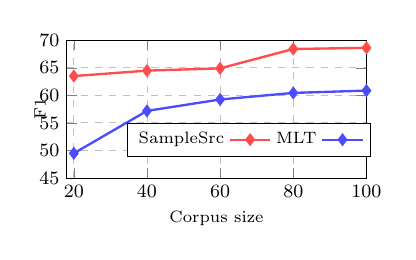
\begin{tikzpicture}[scale = 0.85]
    \footnotesize{
      \begin{axis}[
      ymajorgrids,
  xmajorgrids,
  grid style=dashed,
      width=.50\textwidth,
      height=.30\textwidth,
      legend style={at={(0.20,0.12)}, anchor=south west},
      xlabel={\scriptsize{Corpus size}},
      ylabel={\scriptsize{F1}},
      ylabel style={yshift=-1em},
      xlabel style={yshift=0.0em},
      ymin=45,ymax=70, ytick={45, 50, 55, 60, 65, 70},
      xmin=18,xmax=100,xtick={20, 40, 60, 80, 100},
      legend style={yshift=2pt, legend plot pos=right, legend columns=3 ,font=\scriptsize,cells={anchor=west}}
      ]

    %   \addplot[teal!60,mark=diamond*,line width=1pt, dashed] coordinates {(20,69.81) (40,78.8) (60,80.89) (80,82.01) (100,82.96)};
    %   \addlegendentry{\scriptsize En}
      \addplot[red!70,mark=diamond*,line width=1pt] coordinates {(20,63.52) (40,64.51) (60,64.92) (80,68.44) (100,68.65)};
      \addlegendentry{\scriptsize SampleSrc}
      \addplot[blue!70,mark=diamond*,line width=1pt] coordinates {(20,49.49) (40,57.19) (60,59.27) (80,60.46) (100,60.88)};
      \addlegendentry{\scriptsize MLT}
      \end{axis}
     }
  \end{tikzpicture}
  \caption{{\bf Effect of Source Language Corpus Size.} We report F1-score on all the validation sets.}\label{fig_corpus_size}
\end{figure}

\subsection{Effect of Source Language Corpus Size}
% Here, we investigate the impacts of annotated source language corpus size on DualNER.
In this experiment, we study the impact of annotated source language corpus size on DualNER by sampling different percentages of annotated source language corpus for the Stage 1.
% We sample different percentages of annotated source language corpus used in Stage 1.
% The labels of the remaining annotated source corpus are deleted and used in Stage 2 together with the unlabeled target language text.
Meanwhile, we remove the labels of the remaining source data, and mix it with the unlabeled target language text for the Stage 2.
Figure \ref{fig_corpus_size} shows the comparison between {\it DualNER} and {\it MLT}.
Surprisingly, DualNER trained with only 20\% of annotated source data achieves better performance than MLT trained using complete data, demonstrating the data-efficiency of our proposed method. 

% remove the labels of the rest data, and then use it as unlabeled text  in Stage 2.
% inspected the results of DualNER and {\it MLT} using different size of annotated source language corpus size .
% Specifically, we inspected the results of XX and MLT using different sizes of annotated  


% Thus, we conclude that DualNER can exploit the intrinsic cross-lingual alignment of NER entities among different languages.
% This indicates that our DualNER


% \section{Related Work}

% \paragraph{NER as Different Tasks}
% Although NER is commonly formulated as a sequence labeling task \cite{}, recently other new forms of frameworks have been explored and have shown impressive results.
% For example, \cite{} shift NER from token-level tagging to span-level prediction task while \cite{} conceptualize it as reading comprehension task.
% In this work, we aim to interpret the complementarity between sequence labeling and span prediction.

% \paragraph{Cross-lingual NER}
% There has been growing interest in cross-lingual NER.
% Prior approached can be grouped into two main categories, instance based transfer and model-based transfer.
% Instance-based transfer translates source-language training data to target language, and then apply label projection to annotate the translated data.
% Instead of MT, some earlier approaches also use parallel corpora to construct pseudo training data in the target language \cite{}.
% To minimize resource requirement, \cite{} and \cite{} design frameworks that only rely on word-to-word / phrase-to-phrase translation with bilingual dictionaries.
% Besides, there are also many studies on improving label projection quality with additional feature or better mapping methods \cite{}.
% Different from these methods, our DualNER.

% Model-based transfer directly applies the model trained on the source languge to the target language test data \cite{}, which heavily relies on the quality of cross-lingual representations.
% Recent methods have achieved significant performance improvement by fine-tuning large scale pretrained multilingual LMs \cite{}.
% Besides, there are also some approaches that combine instance-based and model-based transfer \cite{}.
% Compared with these methods, our approach leverages DualNER, and prevents over-fitting on language-specific features by fine-tuning NER models DualNER.

\section{Conclusion}
In this paper, we propose a simple and effective dual-teaching framework, coined DualNER, for zero-shot cross-lingual named entity recognition.
In particular, DualNER makes full use of the exchangeability of the labels in span prediction and sequence labeling, and generates abundant pseudo data for available labeled and unlabeled data.
% to enhance cross-lingual transfer, based on the exchangeability of the labels in span prediction and sequence labeling.
% makes full use of available labeled and unlabeled data to enhance cross-lingual transfer,
Experiments and analysis validate the effectiveness of our DualNER.



\section{Limitations}
The performance of DualNER relies on the capability of cross-lingual transfer of multilingual pretrained models.
% We need a powerful multilingual pretrained model that can conduct target language NER prediction after fine-tuned with annotated source language dataset. 
% Based on a sufficiently good NER model in stage 1, we can generate more reliable
In practice, for an adequate quality of the pseudo-labels generated in the stage 2, it is necessary to ensure that the NER model has acquired certain ability to conduct cross-lingual transfer in the stage 1.

% and thus 
% of to to further boost the cross-lingual NER performance.
% In the second stage in our proposed framework, more reliable pseudo-labels can be generated for the target language text.

% Entries for the entire Anthology, followed by custom entries
\bibliography{anthology,custom}

\appendix

\section{Example of Entity-aware Regularization}
\label{sec:appendix}

\begin{figure}[!h]
\centering
\includegraphics[width=1.0\linewidth]{Regularization.pdf}
\caption{
Entity-aware Regularization.
}
\label{fig_regularization}
\end{figure}

Figure \ref{fig_regularization} illustrates an example of entity-aware regularization.

\section{Settings for Different Pretrained
Models} \label{sec:setting}

\begin{table}[!h]
\centering
\small
\begin{spacing}{1.0}
\begin{tabular}{lcccc}
\toprule
{\bf Model} & {\bf Batch Size} & {\bf Epoch} & {\bf Warmup} & {\bf lr} \\
\midrule
\multicolumn{5}{c}{\bf Stage 1} \\
XLM-R$_{base}$ & 128 & 8 & 300 & 2e-5 \\
InfoXLM$_{large}$ & 128 & 8 & 300 & 2e-5 \\
\midrule
\multicolumn{5}{c}{\bf Stage 2} \\
XLM-R$_{base}$ & 500 & 8 & 300 & 2e-5 \\
InfoXLM$_{large}$ & 128 & 8 & 300 & 2e-5 \\
\bottomrule
\end{tabular}
\end{spacing}
\caption{
\label{tab_settings}
Hyper-parameters settings for different pretrained models.
}
\end{table}

In this paper, we fine-tuned different pretrained models including XLM-R-base and InfoXLM-large.
We evaluate the model each 250 steps.
The batch size, training epoch, warmup steps and learning rate in two-stage training are list in Table \ref{tab_settings}.


% \begin{table*}[!t]
% \centering
% \small
% \begin{spacing}{1.1}
% \resizebox{\textwidth}{22mm}{
% \begin{tabular}{lcccccccccccccccccccc}
% \toprule
% \multicolumn{21}{c}{\textit{InfoXLM_{large}}} \\
% \midrule
% {\bf Method} & en & af & ar & bg & bn & de & el & es & et & eu & fa & fi & fr & he & hl & hu & id & it & ja & jv \\
% CLA & 84.5 & 81.4 & \colorbox{lightgray}{64.2} & 83.2 & \colorbox{lightgray}{78.3} & 81.2 & 81.5 & \colorbox{lightgray}{77.6} & \colorbox{lightgray}{79.0} & \colorbox{lightgray}{67.0} & \colorbox{lightgray}{68.9} & 80.9 & 80.1 & \colorbox{lightgray}{58.0} & 74.1 & \colorbox{lightgray}{82.0} & \colorbox{lightgray}{61.0} & 82.4 & 28.0 & \colorbox{lightgray}{61.2} \\
% SPAN & \colorbox{lightgray}{85.6} & \colorbox{lightgray}{81.7} & 64.2 & \colorbox{lightgray}{84.6} & 77.3 & \colorbox{lightgray}{81.9} & \colorbox{lightgray}{81.9} & 74.3 & 76.6 & 66.4 & 61.2 & \colorbox{lightgray}{82.2} & \colorbox{lightgray}{80.3} & 54.9 & \colorbox{lightgray}{75.1} & 81.4 & 56.8 & \colorbox{lightgray}{82.4} & \colorbox{lightgray}{31.9} & 59.0 \\
% MLT & 85.4 & 83.5 & 62.5 & 84.1 & 78.0 & 80.9 & 82.9 & 80.5 & 78.1 & \colorbox{pink}{\bf 68.3} & 62.6 & 82.4 & 81.6 & 61.2 & 74.8 & 82.5 & 55.8 & 82.4 & 29.9 & 63.9 \\
% DualNER \\
%  \ \ \ \ +TRG_{Trans} & 85.7 & \colorbox{pink}{\bf 83.2} & 65.6 & 84.1 & 80.3 & \colorbox{pink}{\bf 82.8} & 80.9 & 74.5 & \colorbox{pink}{\bf 82.6} & 61.7 & 67.3 & \colorbox{pink}{\bf 82.7} & 82.1 & 66.3 & 77.7 & 82.3 & \colorbox{pink}{\bf 68.1} & \colorbox{pink}{\bf 83.9} & 52.8 & \colorbox{pink}{\bf 68.3} \\
%  \ \ \ \ +TRG_{Gold} & \colorbox{pink}{\bf 85.9} & 82.5 & \colorbox{pink}{\bf 73.5} & \colorbox{pink}{\bf 86.5} & \colorbox{pink}{\bf 82.9} & 81.8 & \colorbox{pink}{\bf 83.0} & \colorbox{pink}{\bf 83.2} & 79.4 & {67.8} & \colorbox{pink}{\bf 71.9} & 82.3 & \colorbox{pink}{\bf 86.3} & \colorbox{pink}{\bf 74.9} & \colorbox{pink}{\bf 79.5} & \colorbox{pink}{\bf 85.3} & {55.1} & 83.7 & \colorbox{pink}{\bf 55.1} & 68.2 \\

% \midrule

% {\bf Method} & ka & kk & ko & ml & mr & ms & my & nl & pt & ru & sw & ta & te & th & tl & tr & ur & vi & yo & zh \\

% CLA & \colorbox{lightgray}{71.7} & 59.9 & \colorbox{lightgray}{60.6} & \colorbox{lightgray}{65.7} & 68.5 & 71.1 & \colorbox{lightgray}{51.8} & 85.4 & 83.3 & 72.0 & 71.6 & \colorbox{lightgray}{61.5} & \colorbox{lightgray}{57.1} & 0.01 & 75.0 & 83.8 & \colorbox{lightgray}{78.2} & 76.6 & 36.4 & 35.0 \\
% SPAN & 71.2 & \colorbox{pink}{60.2} & 57.8 & 64.2 & \colorbox{lightgray}{70.1} & \colorbox{lightgray}{73.3} & 43.9 & \colorbox{lightgray}{86.2} & \colorbox{lightgray}{83.8} & \colorbox{lightgray}{73.6} & \colorbox{lightgray}{72.5} & 60.0 & 51.5 & \colorbox{lightgray}{0.02} & \colorbox{lightgray}{78.0} & \colorbox{lightgray}{85.7} & 75.1 & \colorbox{lightgray}{80.3} & \colorbox{pink}{\bf 56.2} & \colorbox{lightgray}{38.9} \\
% MLT & 74.7 & {56.1} & 61.6 & 68.5 & 67.9 & 72.1 & 46.2 & 86.0 & 83.1 & 74.2 & 72.8 & 61.3 & 54.1 & 0.02 & 76.3 & 84.6 & 75.6 & 78.1 & 43.8 & 36.7 \\
% DualNER \\
%  \ \ \ \ +TRG_{Trans} & 78.6 & 56.1 & 69.3 & 72.6 & \colorbox{pink}{\bf 71.5} & 72.1 & \colorbox{pink}{\bf 68.6} & 86.3 & 85.0 & 72.4 & \colorbox{pink}{\bf 73.3} & 66.2 & 56.5 & 0.05 & \colorbox{pink}{\bf 80.6} & 83.2 & 80.2 & \colorbox{pink}{\bf 83.1} & 42.3 & 55.5 \\
%  \ \ \ \ +TRG_{Gold} & \colorbox{pink}{\bf 79.0} & 51.5 & \colorbox{pink}{\bf 74.2} & \colorbox{pink}{\bf 75.3} & 68.6 & \colorbox{pink}{\bf 74.0} & 66.0 & \colorbox{pink}{\bf 86.7} & \colorbox{pink}{\bf 86.5} & \colorbox{pink}{\bf 80.4} & 71.4 & \colorbox{pink}{\bf 73.6} & \colorbox{pink}{\bf 62.4} & \colorbox{pink}{\bf 0.08} & 76.9 & \colorbox{pink}{\bf 85.9} & \colorbox{pink}{\bf 87.5} & 82.3 & 42.9 & \colorbox{pink}{\bf 57.3} \\
% \bottomrule
% \end{tabular}}
% \end{spacing}
% \caption{
% \label{tab_results_main}
% {\bf Experimental results on the test sets of XTREME-40 NER}. We highlight better results between {\it CLA} and {\it SPAN} with \colorbox{lightgray}{gray} and highlight best results among all methods with \colorbox{pink}{pink}.
% }
% \end{table*}

% \begin{table*}[!t]
% \centering
% \small
% \begin{spacing}{1.0}
% \resizebox{\textwidth}{35mm}{
% \begin{tabular}{lcccccccccccccccccccc}
% \toprule
% \multicolumn{21}{c}{\textit{XLM-R_{base}}} \\
% \midrule
% {\bf Method} & en & af & ar & bg & bn & de & el & es & et & eu & fa & fi & fr & he & hl & hu & id & it & ja & jv \\
% CLA & 81.7 & 75.3 & 49.4 & \colorbox{lightgray}{78.2} & 70.2 & \colorbox{lightgray}{74.4} & 74.7 & 69.5 & \colorbox{lightgray}{71.5} & 58.4 & \colorbox{lightgray}{50.6} & \colorbox{lightgray}{75.6} & 75.3 & \colorbox{lightgray}{52.2} & 68.1 & \colorbox{lightgray}{77.0} & \colorbox{lightgray}{47.7} & 77.2 & 21.5 & 54.8 \\
% SPAN & \colorbox{lightgray}{83.1} & \colorbox{lightgray}{75.8} & \colorbox{lightgray}{51.0} & 77.8 & \colorbox{lightgray}{70.7} & 74.4 & \colorbox{lightgray}{75.4} & \colorbox{pink}{\bf 80.6} & 67.8 & \colorbox{lightgray}{61.8} & 44.5 & 75.3 & \colorbox{lightgray}{79.7} & 50.3 & \colorbox{lightgray}{68.8} & 76.6 & 47.4 & \colorbox{lightgray}{77.9} & \colorbox{lightgray}{25.5} & \colorbox{lightgray}{57.4} \\
% MLT & 82.9 & 75.1 & \colorbox{pink}{\bf 79.3} & 77.6 & 71.3 & 73.6 & 75.2 & 74.3 & 67.8 & 59.8 & 46.6 & 75.3 & 76.5 & 49.7 & 68.3 & 75.1 & 48.8 & 77.0 & 20.1 & 54.2 \\
% FILTER \cite{fang-etal-2021-filter} & 83.3 & 78.7 & 56.2 & 83.3 & 75.4 & 79.0 & 79.7 & 75.6 & 80.0 & 67.0 & \colorbox{pink}{\bf 70.3} & 80.1 & 79.6 & 55.0 & 72.3 & 80.2 & \colorbox{pink}{\bf 52.7} & \colorbox{pink}{\bf 81.6} & 25.2 & 61.8 \\
% DualNER \\
%  \ \ \ \ +TRG_{Trans} & \colorbox{pink}{\bf 84.1} & 78.0 & 59.0 & 80.0 & \colorbox{pink}{\bf 75.5} & 78.1 & 74.7 & 74.5 & 77.1 & 62.4 & 49.8 & 78.6 & 78.9 & 55.7 &  73.3 & 79.5 & 51.0 & {80.0} & 33.8 & 56.4 \\
%  \ \ \ \ +TRG_{Gold} & 83.6 & \colorbox{pink}{\bf 80.0} & 62.4 & \colorbox{pink}{\bf 84.6} & 73.9 & \colorbox{pink}{\bf 81.9} & \colorbox{pink}{\bf 80.8} & {79.1} & \colorbox{pink}{\bf 80.4} & \colorbox{pink}{\bf 68.0} & {66.4} & \colorbox{pink}{\bf 82.9} & \colorbox{pink}{\bf 81.8} & \colorbox{pink}{\bf 69.6} & \colorbox{pink}{\bf 74.3} & \colorbox{pink}{\bf 84.5} & {52.5} & {80.3} & \colorbox{pink}{\bf 38.4} & \colorbox{pink}{\bf 63.5} \\

% \midrule

% {\bf Method} & ka & kk & ko & ml & mr & ms & my & nl & pt & ru & sw & ta & te & th & tl & tr & ur & vi & yo & zh \\
% CLA & \colorbox{lightgray}{66.1} & 42.3 & \colorbox{lightgray}{49.3} & \colorbox{lightgray}{59.3} & \colorbox{lightgray}{61.3} & \colorbox{lightgray}{67.2} & \colorbox{lightgray}{55.2} & 79.8 & 77.0 & \colorbox{lightgray}{64.3} & 67.9 & \colorbox{lightgray}{54.1} & 34.0 & \colorbox{lightgray}{0.04} & 69.7 & 76.7 & 56.0 & \colorbox{lightgray}{68.5} & 37.5 & 26.3 \\
% SPAN & 65.8 & \colorbox{lightgray}{47.8} & 47.7 & 57.4 & 59.4 & 54.3 & 43.0 & \colorbox{lightgray}{80.9} & \colorbox{lightgray}{80.2} & 61.4 & \colorbox{lightgray}{70.7} & 53.8 & \colorbox{lightgray}{47.1} & 0.03 & \colorbox{lightgray}{72.3} & \colorbox{lightgray}{79.3} & \colorbox{lightgray}{66.3} & 66.8 & \colorbox{pink}{\bf 55.8} & \colorbox{lightgray}{31.9} \\
% MLT & 64.5 & 42.8 & 46.7 & 56.3 & 58.8 & 62.3 & 44.2 & 80.5 & 79.3 & 60.8 & 67.6 & 54.6 & 46.2 & 0.01 & 73.0 & 78.1 & 52.9 & 64.9 & 50.2 & 28.4 \\
% FILTER \cite{fang-etal-2021-filter} & 70.0 & 50.6 & \colorbox{pink}{\bf 63.8} & 67.3 & 66.4 & 68.1 & 60.7 & 83.7 & 81.8 & 71.5 & 68.0 & 62.8 & 56.2 & \colorbox{pink}{\bf 1.5} & 74.5 & 80.9 & 71.2 & 76.2 & 40.4 & 35.9 \\
% DualNER \\
%  \ \ \ \ +TRG_{Trans} & 71.7 & 50.0 & 55.7 & 69.4 & 63.6 & \colorbox{pink}{\bf 70.8} & \colorbox{pink}{\bf 67.7} & 83.1 & 80.3 & 63.3 & 70.5 & 58.8 & 50.7 & 0.08 & 78.0 & 81.6 & 63.7 & 73.4 & {37.9} & 43.6 \\
%  \ \ \ \ +TRG_{Gold} & \colorbox{pink}{\bf 74.1} & \colorbox{pink}{\bf 52.2} & {62.7} & \colorbox{pink}{\bf 71.1} & \colorbox{pink}{\bf 72.2} & 70.4 & 66.2 & \colorbox{pink}{\bf 84.6} & \colorbox{pink}{\bf 85.2} & \colorbox{pink}{\bf 64.8} & \colorbox{pink}{\bf 70.7} & \colorbox{pink}{\bf 66.5} & \colorbox{pink}{\bf 61.6} & {0.1} & \colorbox{pink}{\bf 80.2} & \colorbox{pink}{\bf 86.0} & \colorbox{pink}{\bf 84.3} & \colorbox{pink}{\bf 77.2} & 35.6 & \colorbox{pink}{\bf 46.1} \\

% \bottomrule

% \bottomrule
% \multicolumn{21}{c}{\textit{InfoXLM_{large}}} \\
% \midrule
% {\bf Method} & en & af & ar & bg & bn & de & el & es & et & eu & fa & fi & fr & he & hl & hu & id & it & ja & jv \\
% CLA & 84.5 & 81.4 & \colorbox{lightgray}{64.2} & 83.2 & \colorbox{lightgray}{78.3} & 81.2 & 81.5 & \colorbox{lightgray}{77.6} & \colorbox{lightgray}{79.0} & \colorbox{lightgray}{67.0} & \colorbox{lightgray}{68.9} & 80.9 & 80.1 & \colorbox{lightgray}{58.0} & 74.1 & \colorbox{lightgray}{82.0} & \colorbox{lightgray}{61.0} & 82.4 & 28.0 & \colorbox{lightgray}{61.2} \\
% SPAN & \colorbox{lightgray}{85.6} & \colorbox{lightgray}{81.7} & 64.2 & \colorbox{lightgray}{84.6} & 77.3 & \colorbox{lightgray}{81.9} & \colorbox{lightgray}{81.9} & 74.3 & 76.6 & 66.4 & 61.2 & \colorbox{lightgray}{82.2} & \colorbox{lightgray}{80.3} & 54.9 & \colorbox{lightgray}{75.1} & 81.4 & 56.8 & \colorbox{lightgray}{82.4} & \colorbox{lightgray}{31.9} & 59.0 \\
% MLT & 85.4 & 83.5 & 62.5 & 84.1 & 78.0 & 80.9 & 82.9 & 80.5 & 78.1 & \colorbox{pink}{\bf 68.3} & 62.6 & 82.4 & 81.6 & 61.2 & 74.8 & 82.5 & 55.8 & 82.4 & 29.9 & 63.9 \\
% DualNER \\
%  \ \ \ \ +TRG_{Trans} & 85.7 & \colorbox{pink}{\bf 83.2} & 65.6 & 84.1 & 80.3 & \colorbox{pink}{\bf 82.8} & 80.9 & 74.5 & \colorbox{pink}{\bf 82.6} & 61.7 & 67.3 & \colorbox{pink}{\bf 82.7} & 82.1 & 66.3 & 77.7 & 82.3 & \colorbox{pink}{\bf 68.1} & \colorbox{pink}{\bf 83.9} & 52.8 & \colorbox{pink}{\bf 68.3} \\
%  \ \ \ \ +TRG_{Gold} & \colorbox{pink}{\bf 85.9} & 82.5 & \colorbox{pink}{\bf 73.5} & \colorbox{pink}{\bf 86.5} & \colorbox{pink}{\bf 82.9} & 81.8 & \colorbox{pink}{\bf 83.0} & \colorbox{pink}{\bf 83.2} & 79.4 & {67.8} & \colorbox{pink}{\bf 71.9} & 82.3 & \colorbox{pink}{\bf 86.3} & \colorbox{pink}{\bf 74.9} & \colorbox{pink}{\bf 79.5} & \colorbox{pink}{\bf 85.3} & {55.1} & 83.7 & \colorbox{pink}{\bf 55.1} & 68.2 \\

% \midrule

% {\bf Method} & ka & kk & ko & ml & mr & ms & my & nl & pt & ru & sw & ta & te & th & tl & tr & ur & vi & yo & zh \\

% CLA & \colorbox{lightgray}{71.7} & 59.9 & \colorbox{lightgray}{60.6} & \colorbox{lightgray}{65.7} & 68.5 & 71.1 & \colorbox{lightgray}{51.8} & 85.4 & 83.3 & 72.0 & 71.6 & \colorbox{lightgray}{61.5} & \colorbox{lightgray}{57.1} & 0.01 & 75.0 & 83.8 & \colorbox{lightgray}{78.2} & 76.6 & 36.4 & 35.0 \\
% SPAN & 71.2 & \colorbox{pink}{60.2} & 57.8 & 64.2 & \colorbox{lightgray}{70.1} & \colorbox{lightgray}{73.3} & 43.9 & \colorbox{lightgray}{86.2} & \colorbox{lightgray}{83.8} & \colorbox{lightgray}{73.6} & \colorbox{lightgray}{72.5} & 60.0 & 51.5 & \colorbox{lightgray}{0.02} & \colorbox{lightgray}{78.0} & \colorbox{lightgray}{85.7} & 75.1 & \colorbox{lightgray}{80.3} & \colorbox{pink}{\bf 56.2} & \colorbox{lightgray}{38.9} \\
% MLT & 74.7 & {56.1} & 61.6 & 68.5 & 67.9 & 72.1 & 46.2 & 86.0 & 83.1 & 74.2 & 72.8 & 61.3 & 54.1 & 0.02 & 76.3 & 84.6 & 75.6 & 78.1 & 43.8 & 36.7 \\
% DualNER \\
%  \ \ \ \ +TRG_{Trans} & 78.6 & 56.1 & 69.3 & 72.6 & \colorbox{pink}{\bf 71.5} & 72.1 & \colorbox{pink}{\bf 68.6} & 86.3 & 85.0 & 72.4 & \colorbox{pink}{\bf 73.3} & 66.2 & 56.5 & 0.05 & \colorbox{pink}{\bf 80.6} & 83.2 & 80.2 & \colorbox{pink}{\bf 83.1} & 42.3 & 55.5 \\
%  \ \ \ \ +TRG_{Gold} & \colorbox{pink}{\bf 79.0} & 51.5 & \colorbox{pink}{\bf 74.2} & \colorbox{pink}{\bf 75.3} & 68.6 & \colorbox{pink}{\bf 74.0} & 66.0 & \colorbox{pink}{\bf 86.7} & \colorbox{pink}{\bf 86.5} & \colorbox{pink}{\bf 80.4} & 71.4 & \colorbox{pink}{\bf 73.6} & \colorbox{pink}{\bf 62.4} & \colorbox{pink}{\bf 0.08} & 76.9 & \colorbox{pink}{\bf 85.9} & \colorbox{pink}{\bf 87.5} & 82.3 & 42.9 & \colorbox{pink}{\bf 57.3} \\
% \bottomrule
% \end{tabular}}
% \end{spacing}
% \caption{
% \label{tab_results_main}
% {\bf Experimental results on the test sets of XTREME-40 NER}. We highlight better results between {\it CLA} and {\it SPAN} with \colorbox{lightgray}{gray} and highlight best results among all methods with \colorbox{pink}{pink}.
% }
% \end{table*}



\end{document}
